\documentclass[12pt]{article}
\usepackage[usenames,dvipsnames]{color}
\usepackage{listings}
\usepackage{graphicx}
\usepackage{fancyhdr}
\usepackage{framed}
\usepackage[T1]{fontenc}
\usepackage[toc,page]{appendix}
\usepackage[utf8]{inputenc}
\usepackage[brazil]{babel}
\usepackage{fancyvrb}
\usepackage[hmargin=2cm,vmargin=2cm]{geometry}
\usepackage{lastpage}
\usepackage{makeidx}
\pagestyle{fancy}

% cabecalho e rodapé
\setlength{\headheight}{120pt}
\setlength{\textheight}{550pt}
\renewcommand{\headrulewidth}{0pt}
\lhead{
\includegraphics[scale=0.03]{brasao.png}}
\rhead{
\includegraphics[scale=0.4]{logo-pnud.png}}
\cfoot{\textbf{\ProjectCode\ - Inovando a democracia participativa}}
\rfoot{\thepage}

\hyphenation{par-ti-ci-pa-ção}
\bibliographystyle{ieeetr}

% definições sobre o autor e o produto
\newcommand{\MyName}{Joenio Marques da Costa}
\newcommand{\MySurnameForename}{Costa, Joenio}
\newcommand{\SupervisorName}{Gabriella Vieira Oliveira Gonçalves}
\newcommand{\MyEmail}{joenio@colivre.coop.br}
\newcommand{\ContractNumber}{2013/000564}
\newcommand{\ContractYear}{2013}
\newcommand{\ProjectCode}{Projeto BRA/12/018}
\newcommand{\NomeSecretaria}{Secretaria Geral da Presidência da República}
\newcommand{\SiglaSecretaria}{SG/PR}
\newcommand{\ProductNumber}{03}
\newcommand{\ProductTitle}{Proposta de ferramentas de participação social}
\newcommand{\ProductSubtitle}{Ferramenta de elaboração e discussão de
propostas e ferramenta de votação em pares para o Participa.br}
\newcommand{\ProductDescription}{"Documento com proposta para desenvolvimento
  do código de 2 aplicativos para as trilhas de participação social
  priorizados nas reuniões do projeto contendo exemplos e códigos."
}
\newcommand{\ProductValue}{R\$ 18.000,00 (dezoito mil reais)}
\newcommand{\ObjetoContratacao}{"Construção dos códigos para comunidades e
  aplicativos do portal da participação social."
}
\newcommand{\DataEntrega}{25 de Julho de 2014}
\newcommand{\PalavrasChave}{consulta, votação, proposta, colaboração,
ferramentas}

% lista de abreviações
\makeindex

\begin{document}

\newgeometry{hmargin=3cm,vmargin=1.5cm}
\addtolength{\topmargin}{2.5cm}
\thispagestyle{empty}
{\color{MidnightBlue}

{\bf \LARGE Produto \ProductNumber\ -\ \ProductTitle}

\hrulefill

\vspace{1cm}

\begin{center}

{\bf \large Contrato n. \ContractNumber}

\vspace{1.5cm}

{\bf \large Objeto da contratação: \ObjetoContratacao}

\end{center}

\vspace{3.2cm}

Valor do produto: \ProductValue

\vspace{1.2cm}

Data de entrega: \DataEntrega

\vspace{1.2cm}

Nome do consultor: \MyName

\vspace{1.2cm}

Nome do supervisor: \SupervisorName

}

\vspace{2cm}

\begin{center}

\includegraphics[scale=0.04]{brasao.png} \\
{\bf \small \NomeSecretaria}
\end{center}

\restoregeometry
\newpage

\newgeometry{hmargin=3cm,vmargin=1.5cm}
\begin{center}
\thispagestyle{empty}
{\color{MidnightBlue}


\includegraphics[scale=0.9]{logo-pnud.png}

\vspace{4cm}

{\bf \large \ProjectCode\ - Desenvolvimento de Metodologias
de Articulação e Gestão de Políticas Públicas para Promoção da Democracia
Participativa}

\vspace{1.5cm}

{\bf \large Produto \ProductNumber\ -\ \ProductTitle}

\vspace{1.5cm}

\ProductSubtitle

\vspace{4cm}

\MyName

\vspace{2cm}

}


\includegraphics[scale=0.04]{brasao.png} \\
{\bf \small \NomeSecretaria}

\end{center}
\restoregeometry
\newpage

\newgeometry{hmargin=3cm,vmargin=1.5cm}
\addtolength{\topmargin}{2.5cm}
\thispagestyle{empty}
{\color{MidnightBlue}

{\bf \LARGE Produto \ProductNumber\ -\ \ProductTitle}

\hrulefill

\vspace{1cm}

\begin{center}

{\bf \large Contrato n. \ContractNumber}

\vspace{1.5cm}

{\bf \large Objeto da contratação: \ObjetoContratacao}

\end{center}

\vspace{3.2cm}

Valor do produto: \ProductValue

\vspace{1.2cm}

Data de entrega: \DataEntrega

\vspace{1.2cm}

Nome do consultor(a): \MyName

\vspace{1.2cm}

Nome do supervisor(a): \SupervisorName

}

\vspace{2cm}

\begin{center}

\includegraphics[scale=0.04]{brasao.png} \\
{\bf \small \NomeSecretaria}
\end{center}

\restoregeometry
\newpage

\newgeometry{hmargin=3cm,vmargin=1.5cm}
\addtolength{\topmargin}{5cm}
\thispagestyle{empty}

\begin{framed}

{\raggedright \MySurnameForename} \\

\ProductTitle: \ProductSubtitle\ / \ContractYear. \\

Total de folhas: \pageref{LastPage} \\

\vspace{1cm}

Supervisor: \SupervisorName \\

\SiglaSecretaria \\

\NomeSecretaria \\

Palavras-chave: \PalavrasChave. \\

\end{framed}

\vspace{3cm}

{\raggedright 
\includegraphics{licenca-cc-by-nc.png} \ Esta obra é licenciada sob
uma licença Creative Commons - Atribuição-NãoComercial. 4.0 Internacional.}

\restoregeometry
\newpage

\tableofcontents
\newpage

\begin{abstract}
O Participa.br é a plataforma federal de participação social, ela fomenta o
diálogo entre o governo e sociedade civil. É desenvolvida em softwares livres
e utiliza o Noosfero como infraestrutura básica em sua construção. A
plataforma está em constante evolução e este documento traz a proposta de 2
novas ferramentas com diversas novas funcionalidades para promover a
participação do cidadão nas decisões e na elaboração de políticas públicas.

{\bf Palavras-chave:} \PalavrasChave.
\end{abstract}
\newpage

\section{Introdução}

Em consonância com os objetivos e cronograma previsto no âmbito do
projeto BRA/12/018:
\textbf{Desenvolvimento de Metodologias de Articulação e Gestão de
Políticas Públicas para Promoção da Democracia Participativa},
firmado entre a Secretaria-Geral da Presidência da República
(SG/PR) e o Programa das Nações Unidas para o Desenvolvimento (PNUD),
o presente documento apresenta \ProductDescription.

Essa proposta está configurada como produto \ProductNumber~da consultoria técnica
para especificação da construção dos códigos das metodologias de
organização da informação e interação participativa do portal de
participação social, Participa.br, desenvolvido utilizando a ferramenta
Noosfero.

\subsection{O Participa.br}

O Participa.br\cite{participa} é a Plataforma Federal da Participação Social.
Trata-se de mais um espaço para participação social no Brasil, escuta e
diálogo entre o Governo Federal e a Sociedade Civil. 

A plataforma, totalmente desenvolvida em software livre, tem como missão
desenvolver práticas inovadoras de participação via internet e oferta de
espaços de manifestação e debate para qualquer cidadão ou organização, com o
intuito de construir políticas públicas cada vez mais eficazes e efetivas.

O Participa.br é desenvolvido sob a plataforma de software livre para redes
sociais Noosfero e conta com uma equipe multi-disciplinar entre jornalistas,
profissionais de design gráfico, desenvolvedores de software, pesquisadores e
gestores públicos.

\subsection{O Noosfero}

O Noosfero\cite{noosfero} é uma plataforma web livre para redes sociais e de
economia solidária que possui as funcionalidades de Blog, e-Portfolios,
CMS\index{cms}, RSS\index{rss}, discussão temática, agenda de eventos e
inteligência econômica colaborativa em um mesmo sistema. O Noosfero utiliza a
linguagem de programação Ruby\index{ruby} com framework Rails\index{rails}
e suporta bancos de dados, PostgreSQL\index{postgresql}, MySQL, SQLite entre outros.

Ele tem sido desenvolvido desde 2007 como um Software Livre e é licenciado sob
a GNU Affero General Public License (AGPL), versão 3.

\section{Desenvolvimento}

A plataforma de participação social, Participa.br, tem sido desenvolvida desde
de 2013 através de uma metodologia colaborativa e descentralizada, tendo como
ponto central de documentação e gestão de informações a plataforma
Gitlab\cite{gitlab}.

Cada nova ferramenta desenvolvida parte de uma ideia inicial básica e vai
sendo amadurecida através de reuniões presenciais ou remotas entre toda a
equipe, esta ideia gera especificações em forma textual e posteriormente são
transformadas em desenhos, a partir dos quais a equipe de desenvolvimento
inicia seu trabalho.

Este documento traz 2 novas propostas de ferramentas e contará com
especificação textual e modelos visuais que serão posteriormente desenvolvidos
pela equipe de desenvolvedores.

\subsection{Aplicativos para trilhas de participação}
 
O Participa.br utiliza algumas ferramentas como mecanismo de participação,
essas ferramentas permitem aos usuários da rede contribuir através de
comentários, votos ou diretamente sugerindo textos e conteúdos.

Estas ferramentas são organizadas em trilhas de participação, uma trilha
pode utilizar uma ou mais ferramentas e podem ter datas de início e fim de
participação, dando assim um fluxo para a participação social.

Nas próximas seções será apresentado 2 propostas de ferramentas para trilha de
participação.

\subsubsection{Ferramenta para construção e debates de propostas}

Ferramenta proposta inicialmente para atender a consulta de regulamentação do
Marco Civil da Internet baseada em requisitos elaborados pela equipe do
Participa.br em conjunto com o Ministério da Justiça, será desenvolvida como
um plugin Noosfero.

A consulta de regulamentação do Marco Civil da Internet ocorrerá a partir de
grandes temas chamados eixos de debate, nesta ferramenta cada eixo de debate
será exibido junto a uma breve explicação do que ele significa e instruções
básicas de como colaborar. Deve haver também links e artigos relacionados ao
tema sendo exibidos junto a cada eixo, os eixos de debate para regulamentação
do Marco Civil da Internet serão os seguintes:

\begin{enumerate}
  \item Neutralidade de rede
  \item Proteção de dados pessoais
  \item Registros de conexão e acesso a aplicações
  \item Fiscalização e apuração de infrações
  \item Políticas públicas para internet
\end{enumerate}

Os usuários interessados em contribuir para o debate poderão enviar propostas
em cada um destes eixos, estas propostas serão qualitativas e abertas. Os
usuários podem enviar quantas propostas quiserem, as propostas terão o
o seguinte formato (ver Figura~\ref{fig:formulario-proposta}).

\begin{figure}[h]
\center
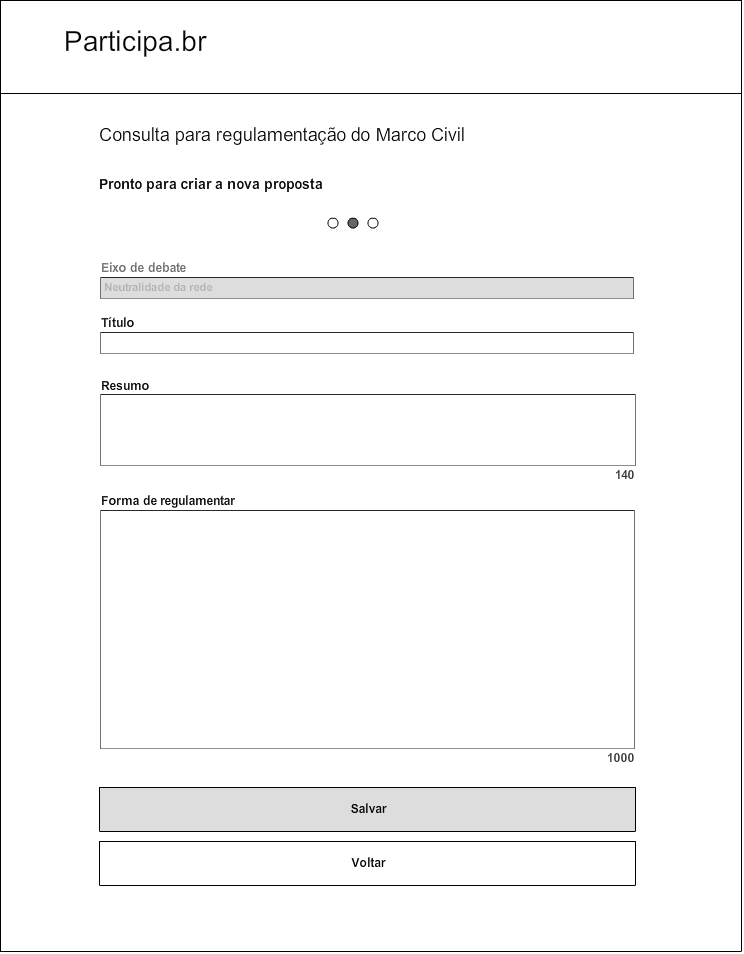
\includegraphics[scale=0.5]{04_-_proposta_passo_2.png}
\caption{Formulário de criação de propostas}
\label{fig:formulario-proposta}
\end{figure}

\begin{itemize}
  \item Título - 70 caracteres - para ajudar na divulgação nas redes sociais
  \item Resumo - 140 caracteres - para ajudar na divulgação nas redes sociais
  \item Forma de regulamentar - 1000 caracteres
\end{itemize}

As propostas irão delimitar os eixos do debate e a discussão sobre cada tema
se dará através da interação dos usuários em cada proposta através de
comentários por parágrafo ou por trecho. Os usuários poderão também concordar
ou discordar da proposta sem a necessidade de fazer comentários.

Os usuários poderão definir tags em seus comentários, estas tags darão
semantica ao comentário indicando que a intenção ali é de incluir ou
excluir um trecho qualquer de texto. A visualização destes comentários
deve levar em consideração a semantica da tag e exibir elementos visuais
que tenham relação com o seu significado.

Sempre que um usuário interagir com uma proposta ele passa a acompanhar as
modificações dela através de seu perfil no Participa.br e pode a qualquer
momento voltar e contribuir com ela.

As propostas de debate em cada eixo formarão uma espécie de fórum de
discussão, mas com uma interface diferenciada e simples, com opções de
ordenação por diversos critérios (ver
Figura~\ref{fig:pagina-inicial}). Exemplos de critérios de ordenação:

\begin{figure}[h]
\center
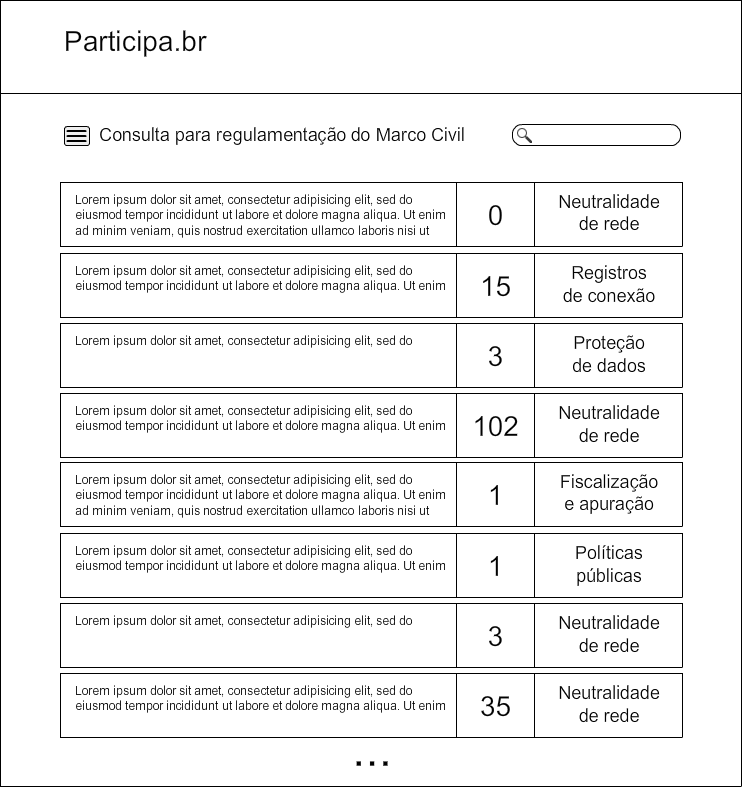
\includegraphics[scale=0.5]{01_-_pagina_inicial.png}
\caption{Proposta da interface da nova ferramenta, página inicial}
\label{fig:pagina-inicial}
\end{figure}

\begin{itemize}
  \item Ordenar de forma aleatória (padrão)
  \item Propostas mais discutidas
  \item Propostas com maior concordancia
  \item Propostas com menor concordancia
\end{itemize}

A interface de criação de propostas deve ser precedida por texto explicativo
de como funciona a consulta e a criação de propostas deve ser dividida em
passos pequenos e simples como pode ser visto das Figuras
\ref{fig:proposta02}, \ref{fig:proposta03} e \ref{fig:proposta04}.

\begin{figure}[h]
\center
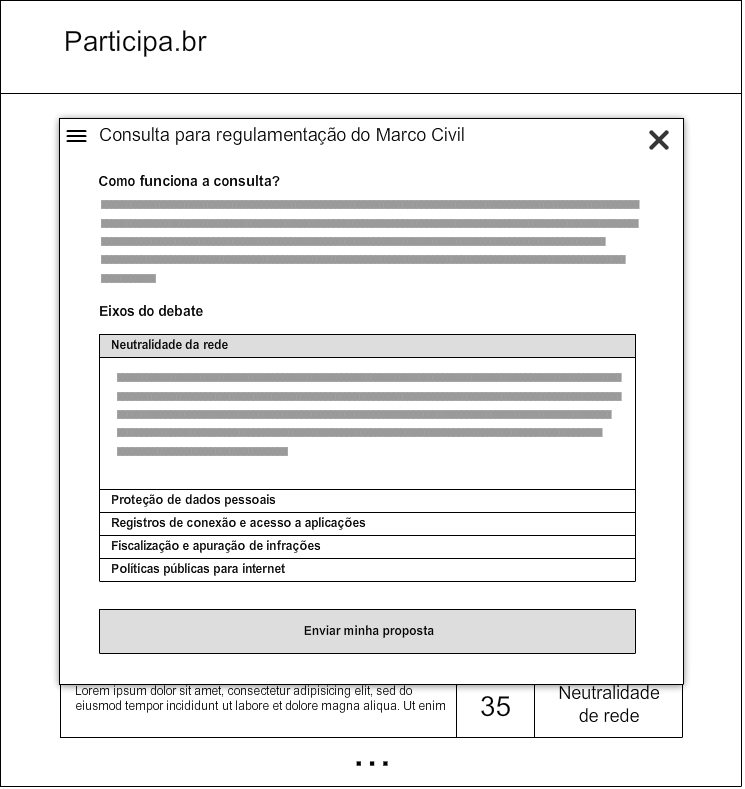
\includegraphics[scale=0.5]{02_-_metodologia_e_eixos.png}
\caption{Proposta da interface da nova ferramenta, como funciona a consulta}
\label{fig:proposta02}
\end{figure}

\begin{figure}[h]
\center
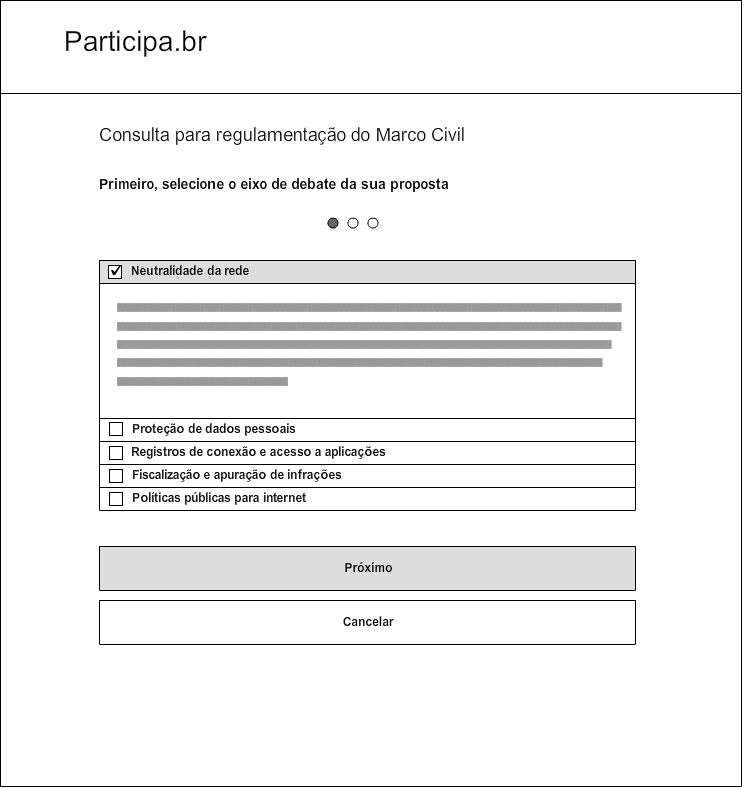
\includegraphics[scale=0.5]{03_-_proposta_passo_1.png}
\caption{Proposta da interface da nova ferramenta, passo 1 da criacao de
propostas}
\label{fig:proposta03}
\end{figure}

\begin{figure}[h]
\center
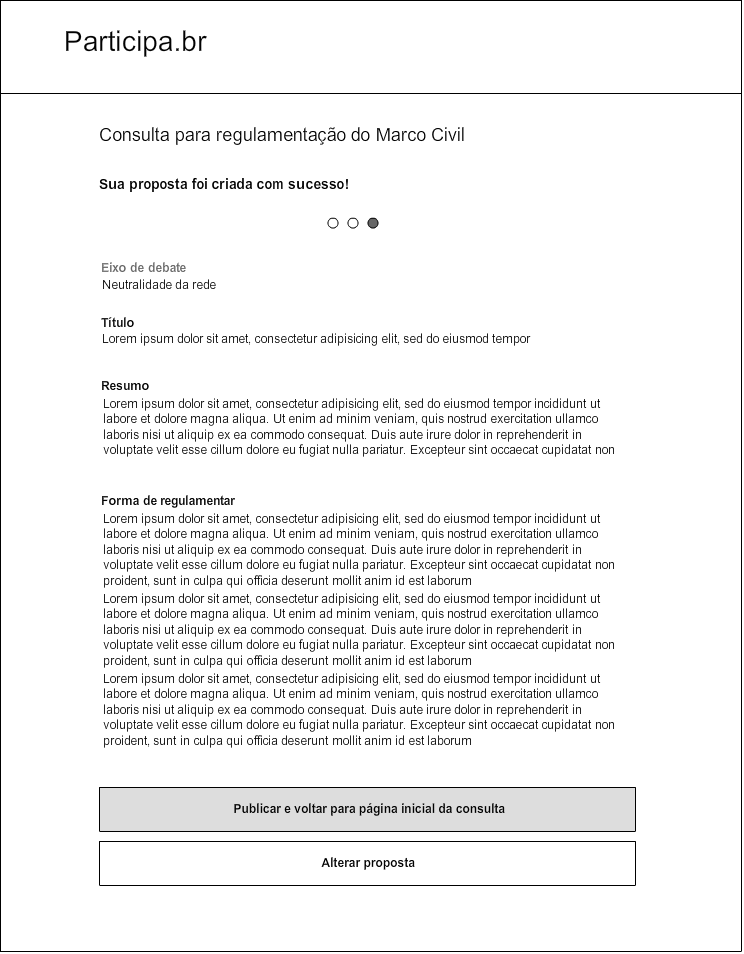
\includegraphics[scale=0.5]{05_-_proposta_passo_final.png}
\caption{Proposta da interface da nova ferramenta, passo 3 da criacao de
propostas}
\label{fig:proposta04}
\end{figure}

A visualização das propostas submetidas pelos usuários será baseada na
interface do Medium\cite{medium}, onde comentários por trecho ou por
parágrafos serão exibidos dinamicamente ao lado de cada trecho ou parágrafo,
como pode ser visto na Figura~\ref{fig:medium}.

\begin{figure}[h]
\center
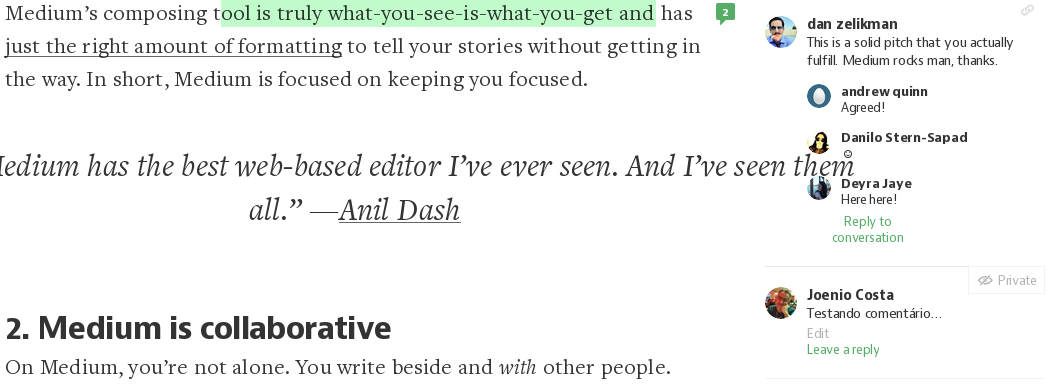
\includegraphics[scale=0.4]{medium.png}
\caption{Proposta de comentários por parágrafo do Medium}
\label{fig:medium}
\end{figure}

\subsubsection{Votação em Pares}

A ferramenta de votação em pares permite grupos de pessoas coletar e priorizar
informações em um processo aberto, democrático e eficiente, esta ferramenta
deve combinar funcionalidades de coleta através de métodos quantitativos e
qualitativos. Deve ser escalável, rápido e permitir quantificar uma pesquisa
enquanto permite inclusão de novas informações pelos participantes.

Além de coletar e priorizar idéias, deve respeitar a privacidade do usuário de
forma que se evite qualquer possibilidade de identificação dos votos. De modo
geral a ferramenta funcionará da seguinte forma:

\begin{itemize}
  \item Administrador cria nova consulta e cadastra idéias para serem votadas
  \item Usuários da plataforma votam através da exibição em pares das
    idéias cadastradas conforme Figura \ref{fig:pairwise}
  \item O usuário pode cadastrar novas idéias, estas novas idéias entrarão
    para moderação
  \item Ao final do período de votação o administrador apura os resultados
    através da uma interface administrativa
\end{itemize}

As propostas de idéias inseridas pelos usuários devem ter limite de caracter e
a interface deve exibir um contador regressivo indicando quantos caracteres o
usuário já digitou, sugere-se um limite de 140 caracteres.

\begin{figure}[h]
\center
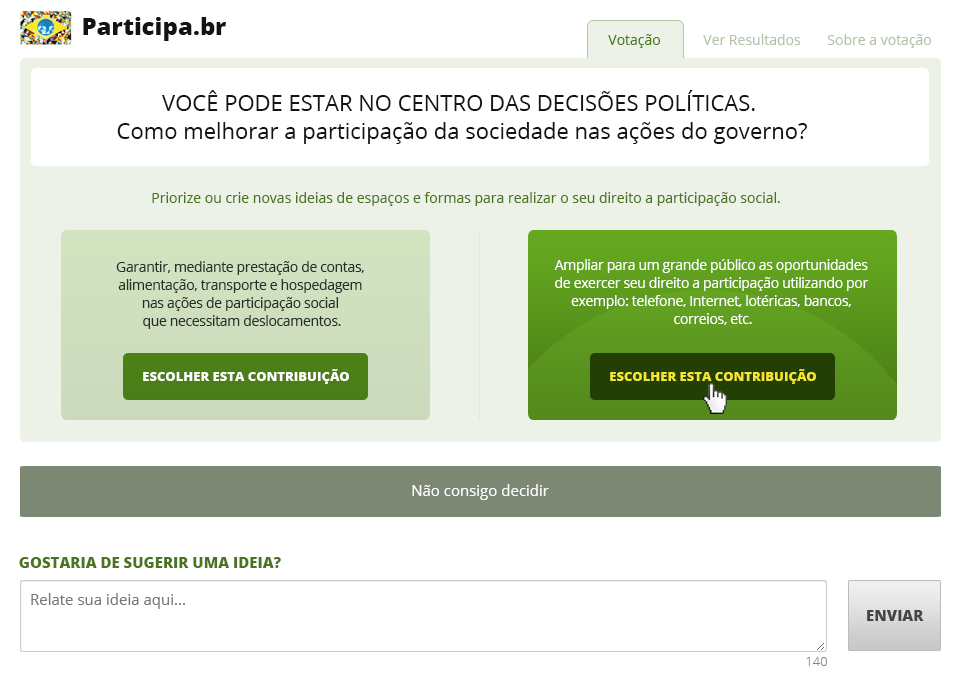
\includegraphics[scale=0.4]{design-votacao-em-pares-verde.png}
\caption{Proposta de interface de votação em pares}
\label{fig:pairwise}
\end{figure}

A implementação desta ferramenta deve gerar código HTML de incorporação em
ambientes externos. Além disso é imprescindível também ter uma interface
alternativa mais simples do mecanismo de votação para incorporação nas redes
sociais, esta interface alternativa não deve ter blocos laterais ou outros
elementos na página.

Para isso será importante aceitarmos votações de usuários não registrados para
os acessos oriundos desses códigos de incorporação externos. Para as votações
dentro do Participa.br, somente usuários cadastrados poderão votar.

Além dos critérios de usabilidade para usuário final é importante ter uma boa
interface de administração contemplando ao menos o seguinte:

\begin{itemize}
  \item Filtros para mediação das ideias cadastradas (ordenar por data, ordem
    alfabetica e nome)
  \item Novas ideias serão sempre mediadas
  \item Área de busca textual nas propostas cadastradas
  \item Busca por usuários cadastrados (para saber quais propostas
    um certo usuário cadastrou)
  \item Possibilidade de aprovação em massa através de checkbox
  \item Possiblidade de agregar duas propostas mantendo os dois autores
\end{itemize}

Esta ferramenta será implementada com base na API\index{api} do pairwise, uma
engine para votação em pares, desenvolvido pela equipe do {\it Trustees of
Princeton University} disponível em:

\begin{itemize}
  \item https://github.com/allourideas/pairwise-api
\end{itemize}

O pairwise é implementado em {\it Ruby\index{ruby} on
Rails\index{rails}}\cite{wikipediaRails} e apesar de ser uma ótima ferramenta
possui uma séria limitação que impede seu uso no Participa.br, que é a
impossibilidade de trabalhar com banco de dados PostgreSQL\index{postgresql}, banco de dados já
em uso no Participa.br.

Além disso será necessário adicionar novos métodos para filtrar e ordenar as
ideias cadastradas pois o pairwise não fornece tal possibilidade e isto é um
requisito necessário para o Participa.br.

O pairwise fornece toda infraestrutura para votação em pares, os dados são
armazenados e recuperados através dele, os algoritmos para cálculo de
relevancia dos votos, toda lógica de negócio fica concentrada nele.

É importante destacar que o Noosfero carece de uma melhoria de performance nos
conteúdos gerados pelos plugins e será necessário otitimizar ao menos um
mecanismo de cache para otimizar o plugin Noosfero do pairwise que será
desenvolvido, o cache será especialmente importante na aba de resultados
da votação.

O plugin Noosfero do pairwise irá implementar uma interface que consome a
API\index{api} do próprio pairwise, o pairwise será instalado e configurado
pela equipe do Participa.br nas mesmas instalações onde hoje está hospedado a
plataforma Noosfero, e este plugin Noosfero irá se comunicar com esta
instancia do pairwise a partir de sua API\index{api}.

\begin{itemize}
  \item https://github.com/allourideas/pairwise-api/wiki/API-Documentation
\end{itemize}

\section{Conclusão}

Neste documento foi apresentado um \ProductDescription

Lembramos que para tornar o Portal de Consulta Pública realmente um canal de
consulta e participação popular na discussão e na definição da agenda
prioritária do país, é necessário que além de documentação faça-se um esforço
de movimentar as pessoar fora do ambiente virtual, para que haja um
engajamento no uso e contribuição deste projeto de forma consistente e perene.

\newpage
\bibliography{bibliografia}
\newpage
\listoffigures
\newpage
\printindex
\newpage
\definecolor{lightgrey}{rgb}{0.95,0.95,0.95}
\lstset{language=Ruby,basicstyle=\small\ttfamily,backgroundcolor=\color{lightgrey}}

\section{Anexos}

\subsection{Exemplo de código do plugin Noosfero para pairwise}

\lstinputlisting{pairwise_content.rb}

\subsection{Exemplo de código XML retornado pelo pairwise-api}

\begin{lstlisting}
<?xml version="1.0" encoding="UTF-8"?>
<prompt>
  <created-at type="datetime">2010-07-01T23:48:01+00:00</created-at>
  <id type="integer">1</id>
  <left-choice-id type="integer">10</left-choice-id>
  <question-id type="integer">7</question-id>
  <right-choice-id type="integer">9</right-choice-id>
  <tracking nil="true"></tracking>
  <updated-at type="datetime">2010-07-01T23:48:01+00:00</updated-at>
  <votes-count type="integer">0</votes-count>
  <left-choice-text>bar</left-choice-text>
  <right-choice-text>foo</right-choice-text>
</prompt>
\end{lstlisting}

\newpage
\appendix
\appendixpage 
\section{Foo bar}
\label{foobar}

%\lstinputlisting{observatorio.rb}


\end{document}
